\documentclass[twocolumn,amsmath,amssymb]{snp}
\pagestyle{empty}
\usepackage{graphicx}% Include figure files
\usepackage{dcolumn}% Align table columns on decimal point
\usepackage{bm}% bold math
\usepackage{amsmath}
\usepackage{ulem}
\topmargin 1.5cm
\textwidth14.5cm
\textheight20cm
\oddsidemargin0.7cm
\columnsep0.2in
\begin{document}
\title{\Large High p$_{T}$ $\Upsilon$(3S) production at LHC energies} 
\author{\large Vineet Kumar}
\email{vineet.salar@gmail.com}
\author{\large Prashant Shukla}
\affiliation{Nuclear Physics Division, Bhabha Atomic Research Centre, Mumbai}
\maketitle
\section*{Introduction}
The quarkonia ($Q\bar Q$) have provided useful tools for probing both 
perturbative and nonperturbative aspects of Quantum Chromodynamics (QCD). 
The quarkonia states are qualitatively different from most other hadrons since 
the velocity of the heavy constituents is small allowing a 
non-relativistic treatment of bound states. The NRQCD formalism is one 
of the most promising theoretical framework for the study of heavy quarkonium 
production~\cite{Bodwin:1994jh}. The study of the differential charmonia production 
cross sections in high energy p+p collisions is completed using 
NRQCD formalism~\cite{Kumar:2016ojy}.
\section*{Bottomonia Production in p$+$p collisions}
Under NRQCD, the cross-section for direct production of a resonance $H$ in 
a collision of particles $A$ and $B$ can be expressed in factorized form 
\begin{equation}
  \begin{split}
    &E\frac{d^{3}\sigma^{ab\rightarrow cd}}{d^{3}p}(^{(2S+1)}L_{J}) = \sum_{a,b}\int dx_a\,dx_b \\
    &G_{a/A}(x_a,\mu_{F}^{2}) G_{b/B}(x_b,\mu_{F}^{2})\frac{\hat s}{\pi}\frac{d\sigma}{d\hat t}\\
    &(ab\rightarrow^{(2S+1)}L_{J}c)\cdot \delta(\hat s + \hat t + \hat u -M^{2}) \nonumber
\end{split}
\end{equation}
where, $G_{a/A}(G_{b/B})$ is the parton distribution function (PDF) of the incoming parton $a(b)$ in the 
incident hadron $A(B)$, which depends on the momentum fraction $x_a(x_b)$ and the factorization 
scale $\mu_F$. The short distance contribution $d\sigma/d\hat t$ can be calculated 
within the framework of perturbative QCD (pQCD). $(ab\rightarrow^{(2S+1)}L_{J}c)$ 
represents the probability of evolving a bound quarkonia state from a Q$\overline{\rm Q}$
pair. These probabilities (LDMEs) should be estimated from the experimental measurements. 
In this work the production cross section of b$\overline{\rm b}$ bound states is calculated 
in p$+$p collisions $\sqrt{s}$ = 7 TeV and measured data from CMS and ATLAS 
collaborations~\cite{Khachatryan:2015qpa,Aad:2012dlq} is used to constrain the LDMEs required for
$\Upsilon$(3S) production.
%\begin{figure}
%  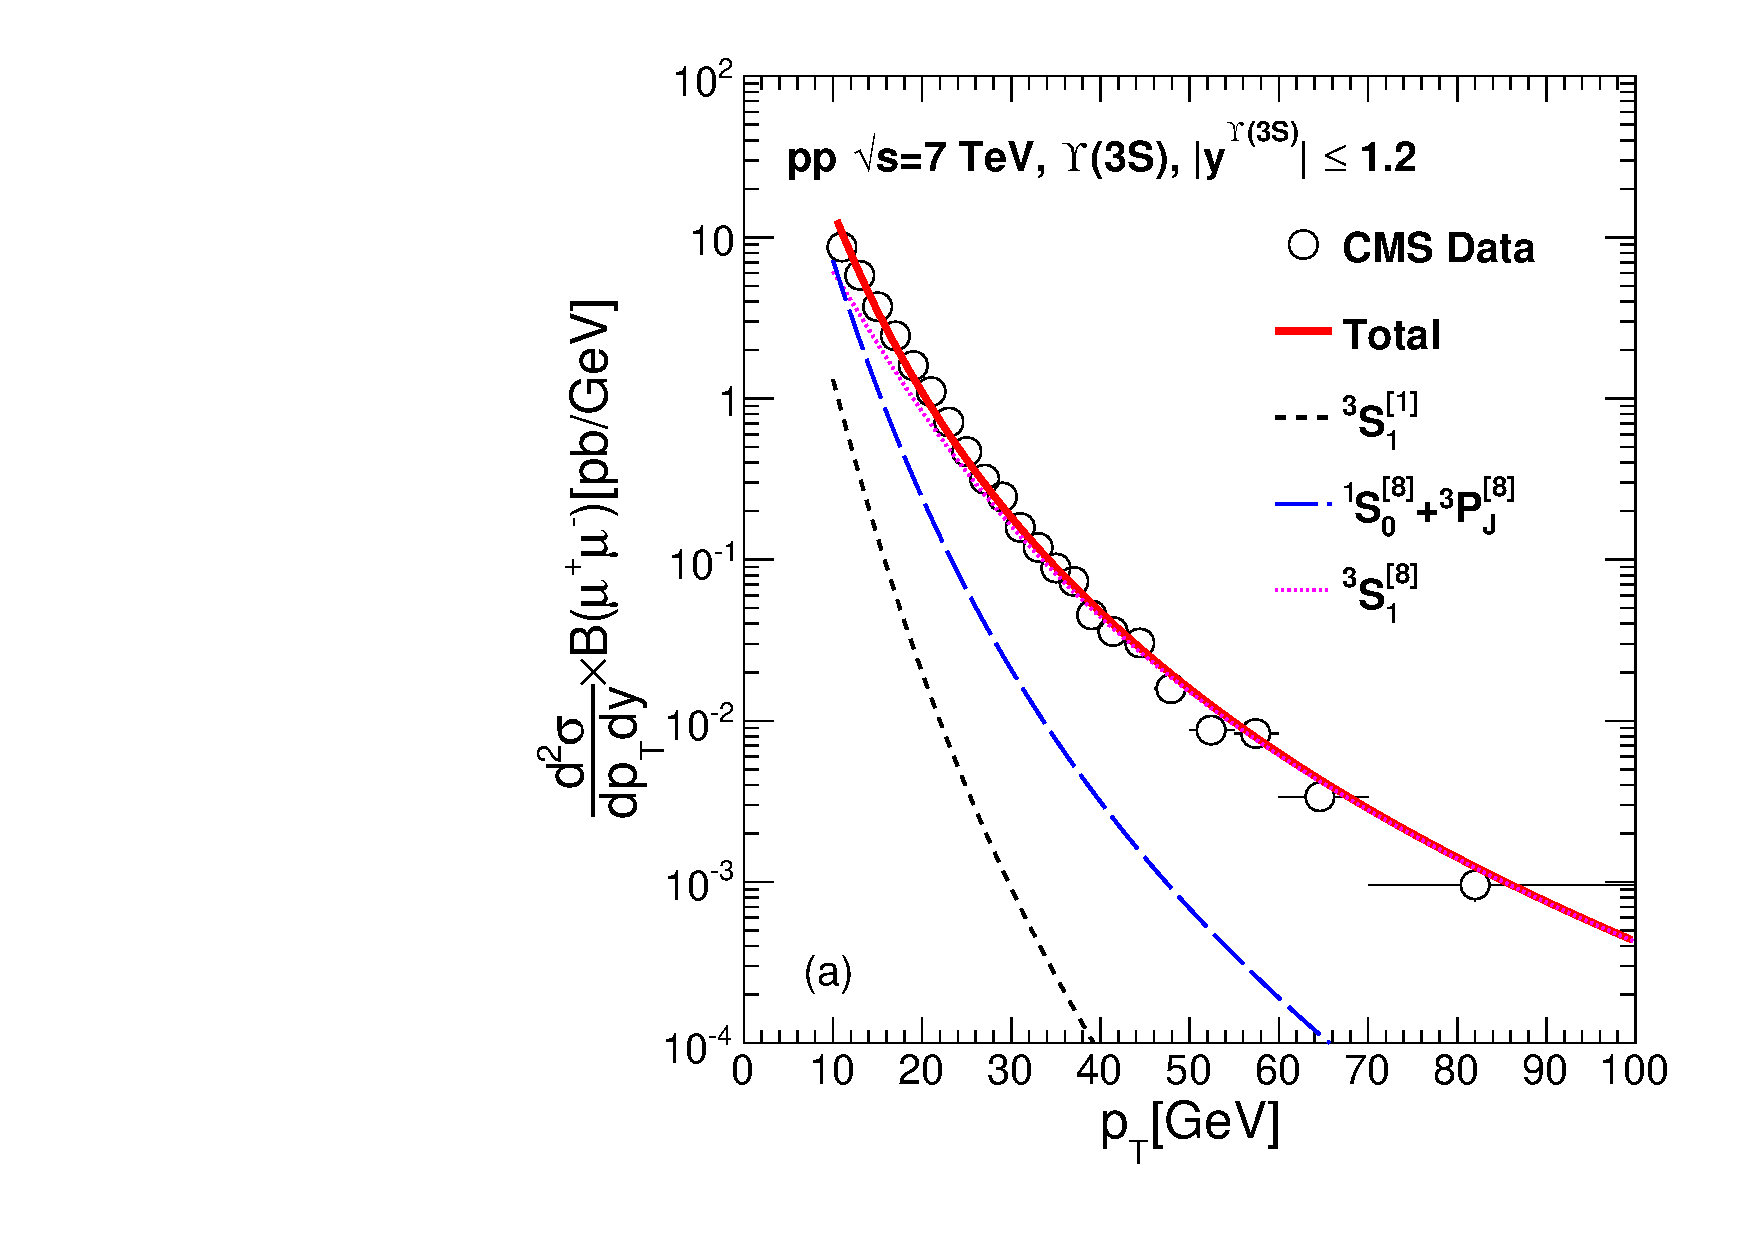
\includegraphics[width=0.39\textwidth]{Fig1_Y3S_CMS.pdf}
%  \caption{The NRQCD calculations of production cross section of $\Upsilon$(3S) in p+p collisions 
%    as a function of transverse momentum compared with the measured CMS data at $\sqrt{s}$ = 7 
%    TeV~\cite{Khachatryan:2015qpa}. The LDMEs are obtained by a combined fit of the 
%    CMS and ATLAS data.}
%  \label{Fig:SigmaY3SCMS}
%\end{figure}
%\begin{figure}
%  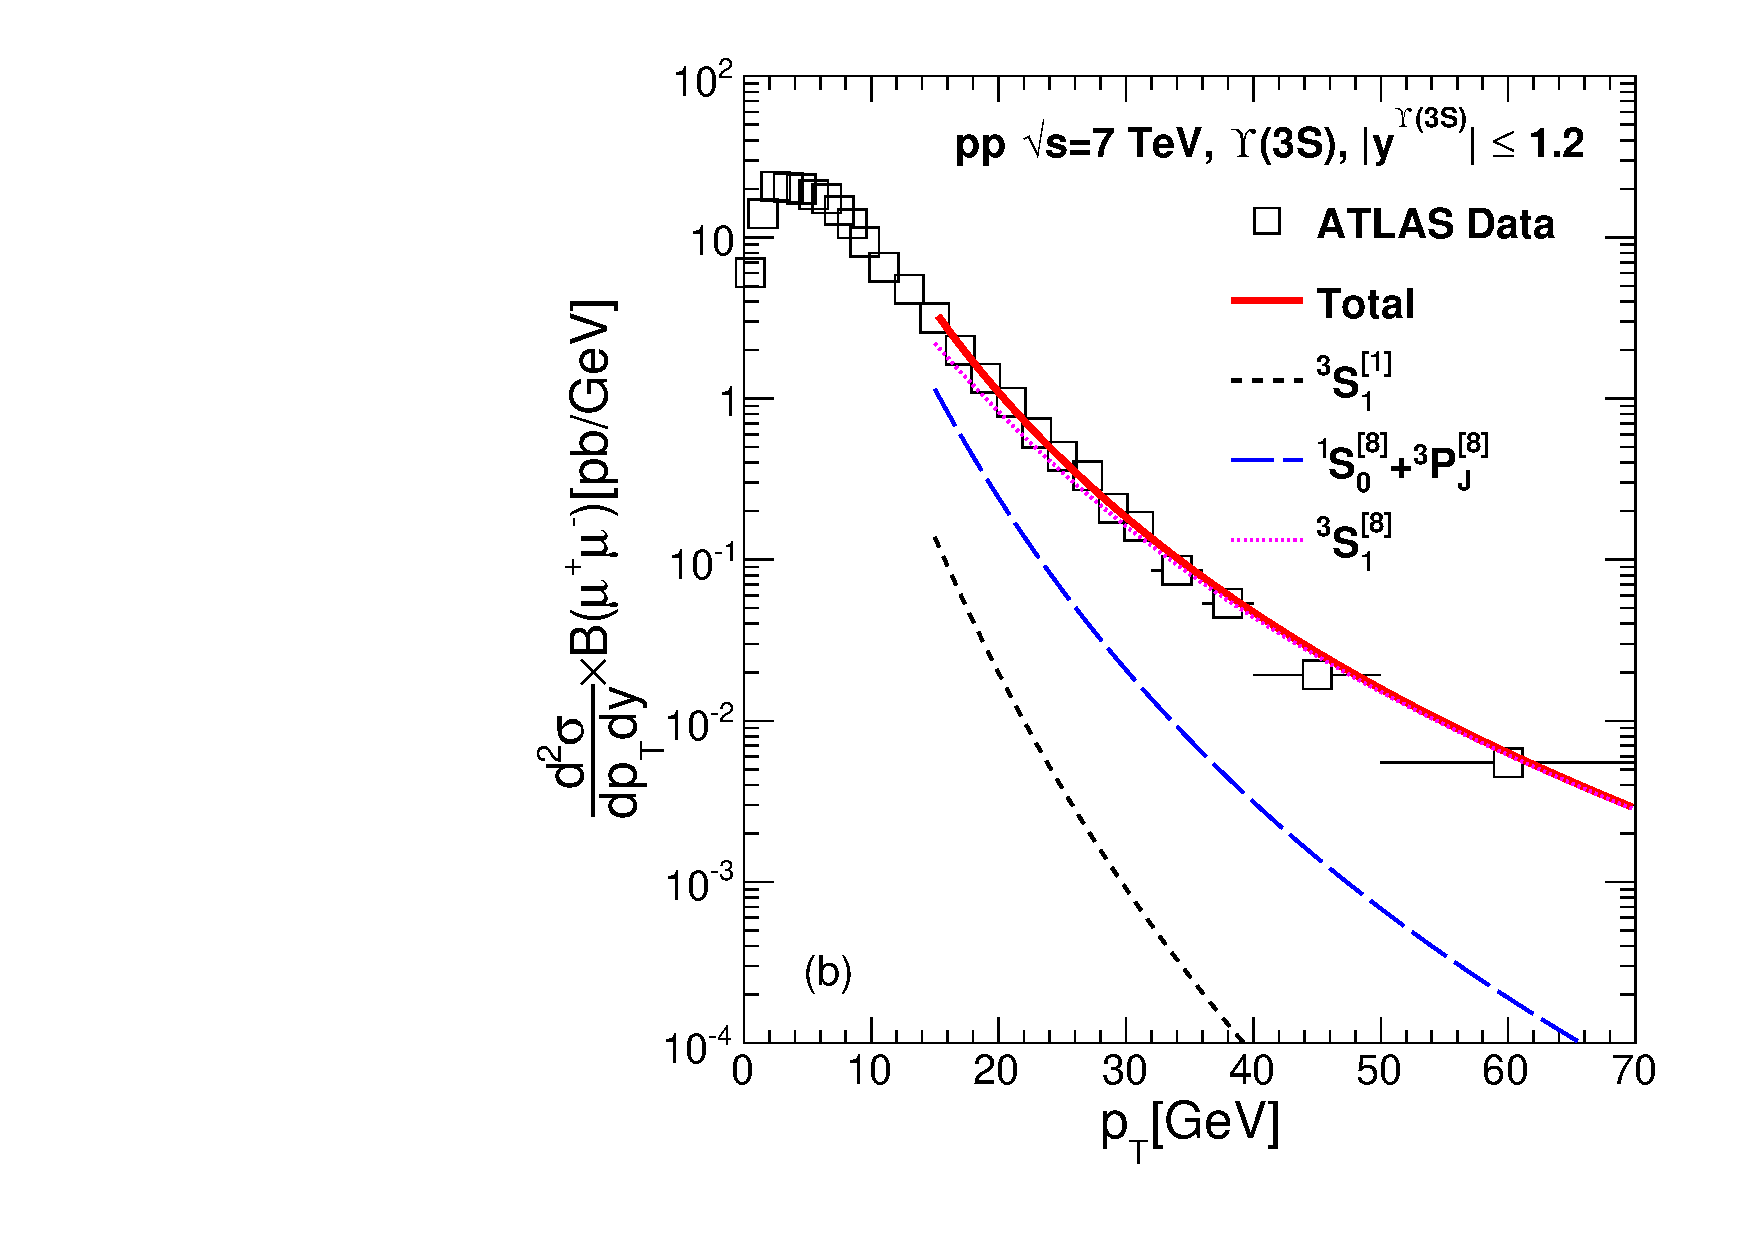
\includegraphics[width=0.39\textwidth]{Fig2_Y3S_ATLAS.pdf}
%  \caption{The NRQCD calculations of production cross section of $\Upsilon$(3S) in p+p collisions 
%    as a function of transverse momentum compared with the measured ATLAS data at $\sqrt{s}$ = 7 
%    TeV~\cite{Aad:2012dlq}. The LDMEs are obtained by a combined fit of the 
%    CMS and ATLAS data.}
%  \label{Fig:SigmaY3SATLAS}
%\end{figure}
\begin{figure}
  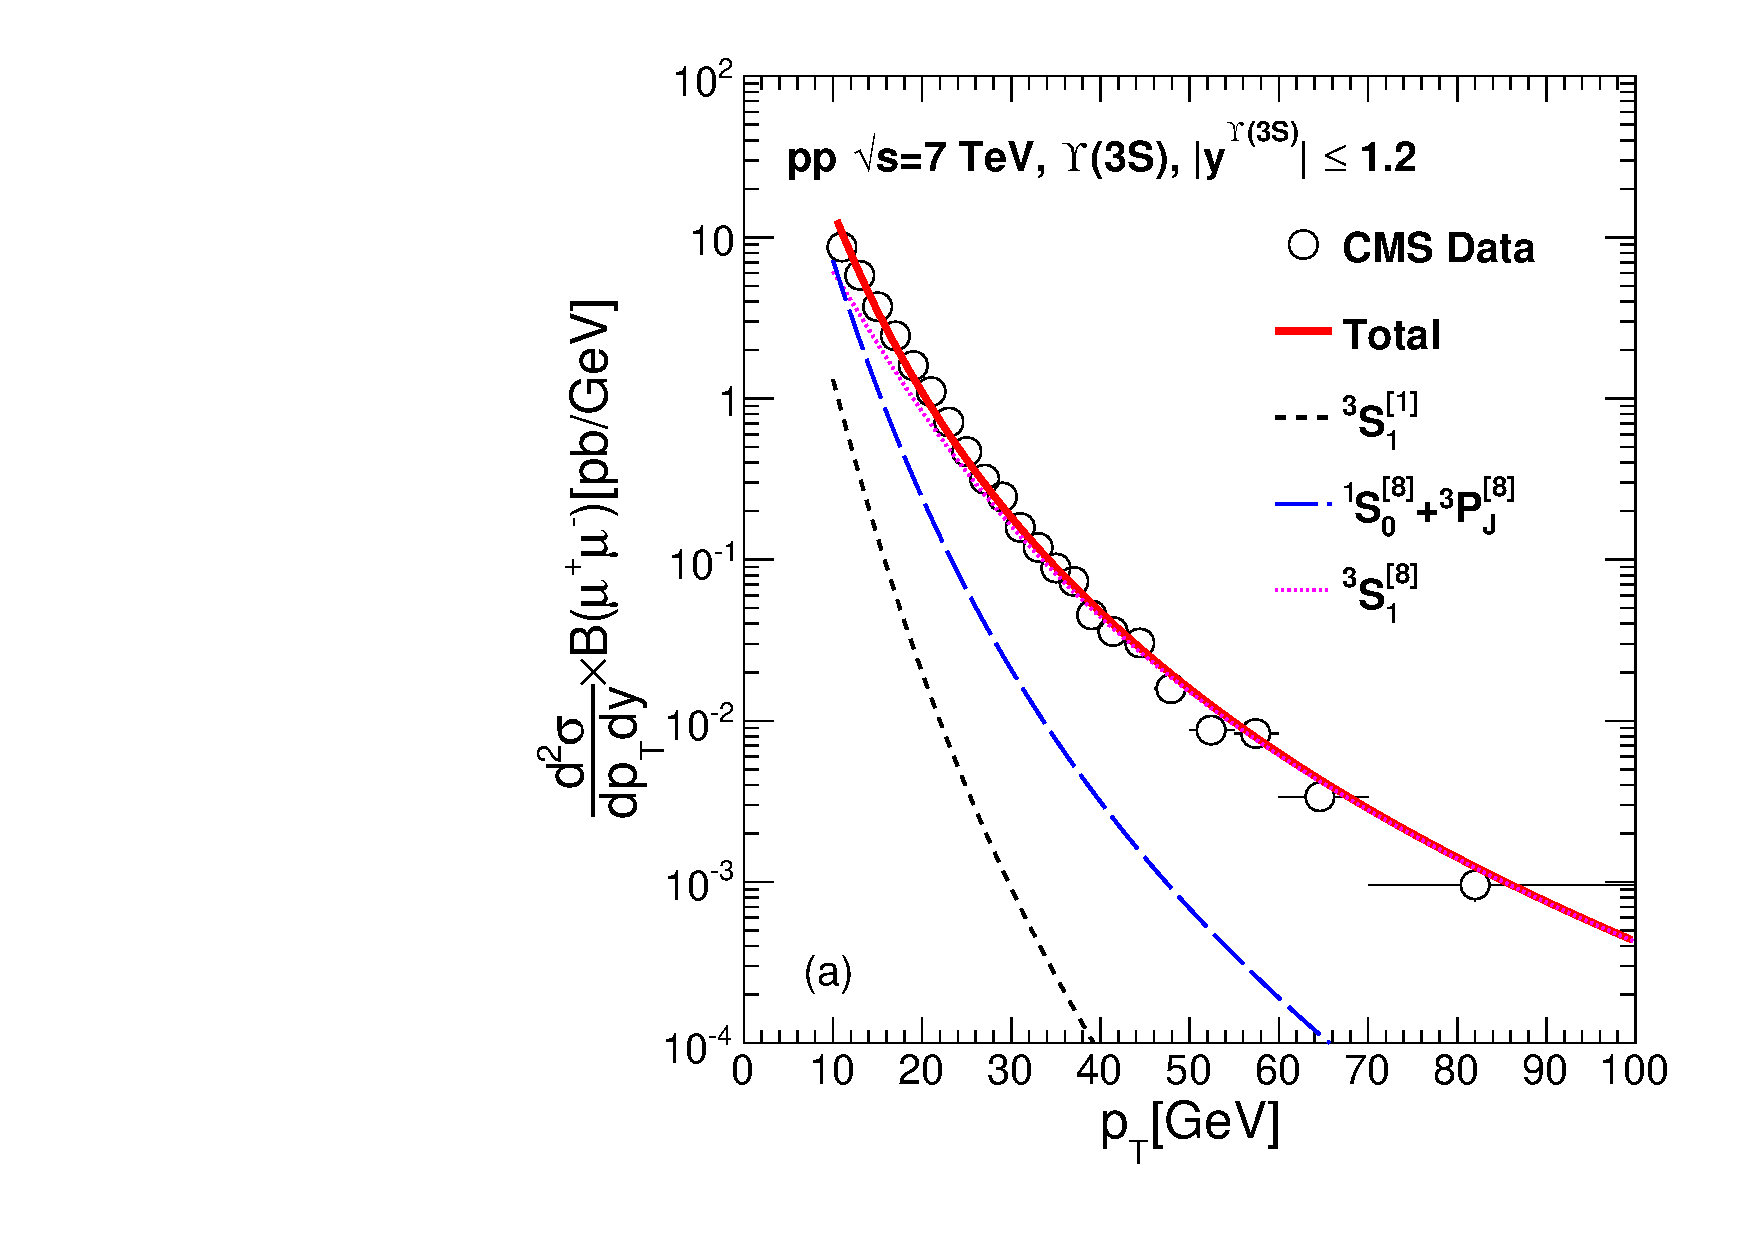
\includegraphics[width=0.43\textwidth]{Fig1_Y3S_CMS.pdf}
  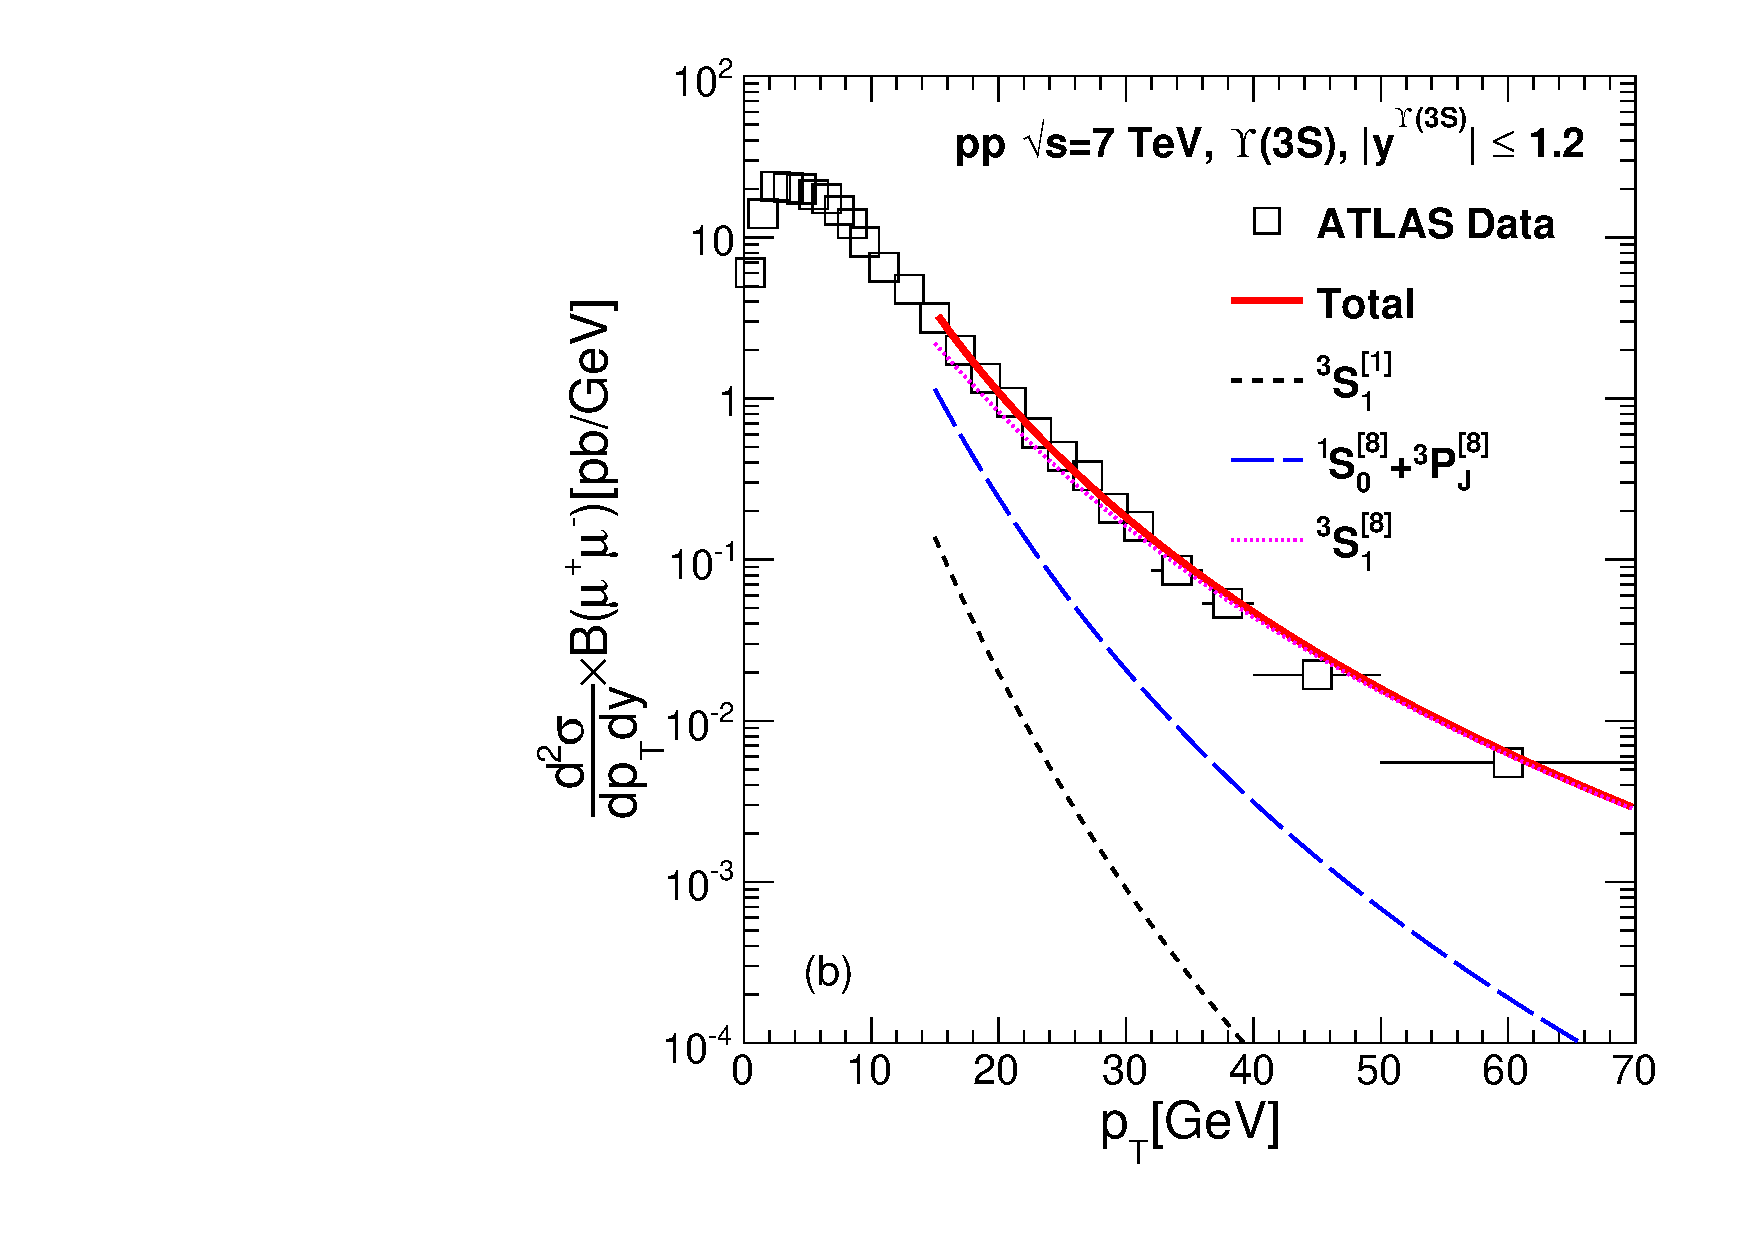
\includegraphics[width=0.43\textwidth]{Fig2_Y3S_ATLAS.pdf} 
 \caption{The NRQCD calculations of production cross section of $\Upsilon$(3S) in p+p collisions at 
   $\sqrt{s}$ = 7 TeV, as a function of transverse momentum compared with the measured data 
   at CMS~\cite{Khachatryan:2015qpa} and ATLAS~\cite{Aad:2012dlq} experiment. The LDMEs are obtained by 
   a combined fit of the CMS and ATLAS data.}
  \label{Fig:SigmaY3SCMS}
\end{figure}
The LDMEs are predicted to scale with a definite power of the relative velocity $v$ of the heavy constituents 
inside $Q\bar Q$ bound states. In the limit $v<<1$, the production of quarkonium is based on the $^3S_1^{[1]}$ 
and $^3P_J^{[1]}$ ($J$ = 0,1,2) Color Singlet states, $^1S_0^{[8]}$, $^3S_1^{[8]}$ and $^3P_J^{[8]}$ Color 
Octet states.  The differential cross section for the direct production of $\Upsilon$(3S) can be written as the 
sum of these contributions,
\begin{eqnarray}
d\sigma(\Upsilon(3S)) &= d\sigma(Q\overline{Q}([^3S_1]_{1}))
                   \,M_{L}([^3S_1]_{1}) \nonumber \\
                &+\, d\sigma(Q\overline{Q}[^1S_0]_{8}))
                   \,M_{L}([^1S_0]_{8}) \nonumber \\ 
                &+ \, d\sigma(Q\overline{Q}([^3S_1]_{8}))
                   \,M_{L}([^3S_1]_{8}) \nonumber \\
                &+ \, d\sigma(Q\overline{Q}([^3P_J]_{8}))
                   \,M_{L}([^3P_0]_{8})\nonumber \\ \nonumber
                %&+  d\sigma(Q\overline{Q}([^3P_1]_{8}))
                 %  \,M_{L}([^3P_1]_{8})\\
                %&+  d\sigma(Q\overline{Q}([^3P_2]_{8}))
                 %  \,M_{L}([^3P_2]_{8})\\
\label{eq:dsigmaJ}
\end{eqnarray}
In our calculations, we used the expressions for the short distance cross-sections 
from Refs.~\cite{Baier:1983va,Cho:1995vh}.
\section*{Results and discussion}
$\Upsilon$(3S) is the highest known bound state in the b$\overline{\rm b}$ spectrum 
so it must not have any feed down contribution. 
The expressions and the values for the 
color-singlet LDMEs can be obtained by solving the non-relativistic 
wavefunctions~\cite{Cho:1995vh}. 
The CO LDMEs can not be related to the non-relativistic
wavefunctions of $b \bar b$ since it involves a higher Fock state and thus
measured data~\cite{Khachatryan:2015qpa,Aad:2012dlq} is used to constrain them.
Figure~\ref{Fig:SigmaY3SCMS} shows the NRQCD calculations of production cross section of 
$\Upsilon$(3S) in p+p collisions as a function of transverse momentum compared with the 
measured data in CMS~\cite{Khachatryan:2015qpa} and ATLAS~\cite{Khachatryan:2015qpa} 
detectors at LHC. 
%Figure~\ref{Fig:SigmaY3SATLAS} shows the same for ATLAS~\cite{Aad:2012dlq}. 
% NRQCD calculations of production cross section of 
%$\Upsilon$(3S) in p+p collisions as a function of transverse momentum compared with the 
%measured data in ATLAS detector at LHC~\cite{Aad:2012dlq}.
The color-singlet contribution along with the calculated value 
and color-octet contributions fitted from data are given below for the 
$\Upsilon$(3S) production.
\begin{eqnarray}
  &M_{L}([^3S_1]_{1}) &= 4.3 \,{\rm GeV^3}\nonumber \\
  &M_{L}([^3S_1]_{8}) &= (0.0725\pm0.0013) \, {\rm GeV^3}\nonumber \\
  &M_{L}([^1S_0]_{8}) &= (0.0126\pm0.0008) \,{\rm GeV^3} \nonumber \\ \nonumber
  &&=  M_{L}([^3P_0]_{8})/5m_{b}^{2}\,\,{\rm GeV^3} \nonumber \\ \nonumber
\end{eqnarray}
The combined fitting of CMS and ATLAS data is done to extract common color octet LDMEs 
those explain both the datasets simultaneously. The $\chi^2/dof$ is 3.25 for the 
combined fitting. Our value of $M_{L}([^3S_1]_{8})$ is compatible with the value obtained in the recent 
calculations~\cite{Sharma:2012dy} while the value of $M_{L}([^1S_0]_{8})$ is larger than
the value of Ref.~\cite{Sharma:2012dy}. We significantly improve the large ($\approx 300\%$) error 
present on the value of $M_{L}([^1S_0]_{8})$ in Ref.~\cite{Sharma:2012dy}, by using combined 
fitting and latest LHC data.
\section*{Summary}
We have calculated the differential production cross-section of $\Upsilon$(3S) meson
as a function of transverse momentum. The data from LHC experiments are used to 
obtain the values of color octet LDMEs. We plan to present a rigorous study of 
production of all states of bottomonia at LHC energies using NRQCD.
The reevaluation of all LDMEs required for bottomonia production is in progress using 
latest data from LHC.         
\begin{thebibliography}{50}
\bibitem{Bodwin:1994jh}
G.~T.~Bodwin, E.~Braaten, and G.~P.~Lepage,
%``Rigorous QCD analysis of inclusive annihilation and production of heavy
%quarkonium,''
Phys.\ Rev.\ D {\bf 51} 1125 (1995), 
[Erratum-ibid.\ D {\bf 55} 5853 (1997)].
\bibitem{Kumar:2016ojy} 
  V.~Kumar and P.~Shukla,
  %``Charmonia production in p+p collisions under NRQCD formalism,''
  arXiv:1606.08265 [hep-ph].
  %%CITATION = ARXIV:1606.08265;%%
\bibitem{Khachatryan:2015qpa} 
  V.~Khachatryan {\it et al.} [CMS Collaboration],
%  ``Measurements of the $\Upsilon$(1S), $\Upsilon$(2S), and $\Upsilon$(3S) differential 
%  cross sections in pp collisions at $\sqrt{s} =$ 7 TeV,''
  Phys.\ Lett.\ B {\bf 749}, 14 (2015),[arXiv:1501.07750 [hep-ex]].
\bibitem{Aad:2012dlq} 
  G.~Aad {\it et al.} [ATLAS Collaboration],
 % ``Measurement of Upsilon production in 7 TeV pp collisions at ATLAS,''
  Phys.\ Rev.\ D {\bf 87}, no. 5, 052004 (2013),
  [arXiv:1211.7255 [hep-ex]].
%\bibitem{Owens:1986mp} 
%  J.~F.~Owens,
%  %``Large Momentum Transfer Production of Direct Photons, Jets, and Particles,''
%  Rev.\ Mod.\ Phys.\  {\bf 59}, 465 (1987).
%\bibitem{Lai:2010vv} 
%  H.~L.~Lai {\it et al.} %, M.~Guzzi, J.~Huston, Z.~Li, P.~M.~Nadolsky, J.~Pumplin and C.-P.~Yuan,
%  %``New parton distributions for collider physics,''
%  Phys.\ Rev.\ D {\bf 82}, 074024 (2010).
%  %[arXiv:1007.2241 [hep-ph]].
\bibitem{Baier:1983va} 
  R.~Baier and R.~Ruckl,
  %``Hadronic Collisions: A Quarkonium Factory,''
  Z.\ Phys.\ C {\bf 19}, 251 (1983).
%\bibitem{Humpert:1986cy} 
%  B.~Humpert,
%  %``Narrow Heavy Resonance Production By Gluons,''
%  Phys.\ Lett.\ B {\bf 184}, 105 (1987).
%\bibitem{Gastmans:1987be} 
%  R.~Gastmans, W.~Troost and T.~T.~Wu,
%  %``Production of Heavy Quarkonia From Gluons,''
%  Nucl.\ Phys.\ B {\bf 291}, 731 (1987).
\bibitem{Cho:1995vh} 
  P.~L.~Cho and A.~K.~Leibovich,
  %``Color octet quarkonia production,''
  Phys.\ Rev.\ D {\bf 53}, 150 (1996).
  %[hep-ph/9505329].
%\bibitem{Cho:1995ce} 
%  P.~L.~Cho and A.~K.~Leibovich,
%  %``Color octet quarkonia production. 2.,''
%  Phys.\ Rev.\ D {\bf 53}, 6203 (1996).
%  %[hep-ph/9511315].
%\bibitem{Chatrchyan:2011kc} 
%  S.~Chatrchyan {\it et al.} [CMS Collaboration],
%  %``$J/\psi$ and $\psi_{2S}$ production in $pp$ collisions at $\sqrt{s}=7$ TeV,''
%  JHEP {\bf 1202}, 011 (2012).
%%[arXiv:1111.1557 [hep-ex]].
%\bibitem{Khachatryan:2015rra} 
%  V.~Khachatryan {\it et al.} [CMS Collaboration],
%  %``Measurement of J/ψ and ψ(2S) Prompt Double-Differential Cross Sections in pp Collisions at $\sqrt{s}$=7  TeV,''
%  Phys.\ Rev.\ Lett.\  {\bf 114}, no. 19, 191802 (2015).
%  %[arXiv:1502.04155 [hep-ex]].
\bibitem{Sharma:2012dy} 
  R.~Sharma and I.~Vitev,
  %``High transverse momentum quarkonium production and dissociation in heavy ion collisions,''
  Phys.\ Rev.\ C {\bf 87}, 044905 (2013).
%  [arXiv:1203.0329 [hep-ph]].
\end{thebibliography}

\end{document}
